\chapter{Réseaux programmables avec SDN}

Le but de ce chapitre est de (re)définir SDN et de présenter en quoi SDN répond aux besoins explicités dans le chapitre 1.
Ce chapitre répond aux questions : Qu'est-ce que SDN ? Qu'est-ce que se la propose ? Où on en est par rapport à SDN ?

\section{Séparation de l'intelligence (contrôle) de la commutation}

blabla...
On cherche à concevoir une architecture plus adaptée aux enjeux de la communication de l'actualité discutés dans le chapitre 1. Cette problématique a amené scientistes et les ingénieurs impliqués à concevoir \gls{sdn}. \gls{sdn} est un nouveau \glslink{paradigme}{paradigme} réseau qu'on est actuellement en cours de développer pour adapter l'infrastructure existante au nouveau scénario.


%SDN is described in this article with the Open Networking Foundation (ONF) [1] definition: “In the SDN architecture, the control and data planes are decoupled, network intelli- gence and state are logically centralized, and the underlying network infrastructure is abstracted from the applications.”

SDN est défini au long de l'article par  selon \gls{onf} \cite{SDNNewNormONFExecutiveSummary} : Dans l'architecture SDN, les plans de contrôle et de données sont découpés, l'intelligence et l'état du réseau sont logiquement centralisés, et l'infrastructure du réseau est donc abstraite des applications. 

[déf plan de controle]. [Déf plan de donnés]


\begin{figure}[!h] %on ouvre l'environnement figure
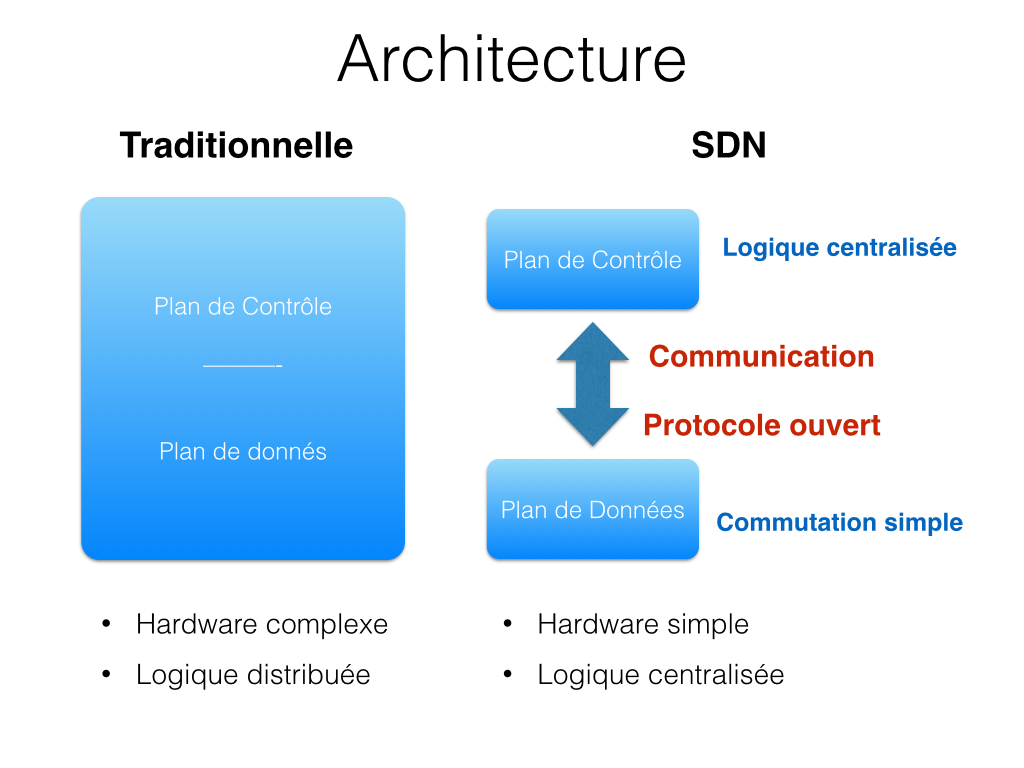
\includegraphics[width=15cm]{images/ComparaisonArchis.png} %ou image.png, .jpeg etc.
\caption{ Architecture Traditionnelle et SDN} %la légende
\label{image_soleil} %l'étiquette pour faire référence à cette image
\end{figure} %on ferme l'environnement figure

\clearpage

\section{Tableaux de flux}

\section{Contrôleur}

\section{Un point sur la situation}
\subsection{ONF}

\subsection{OpenFlow - Protocoles standardisés}
